\section{Design of XXX}
\label{sec:design}
\begin{figure}[t]
  \centering
  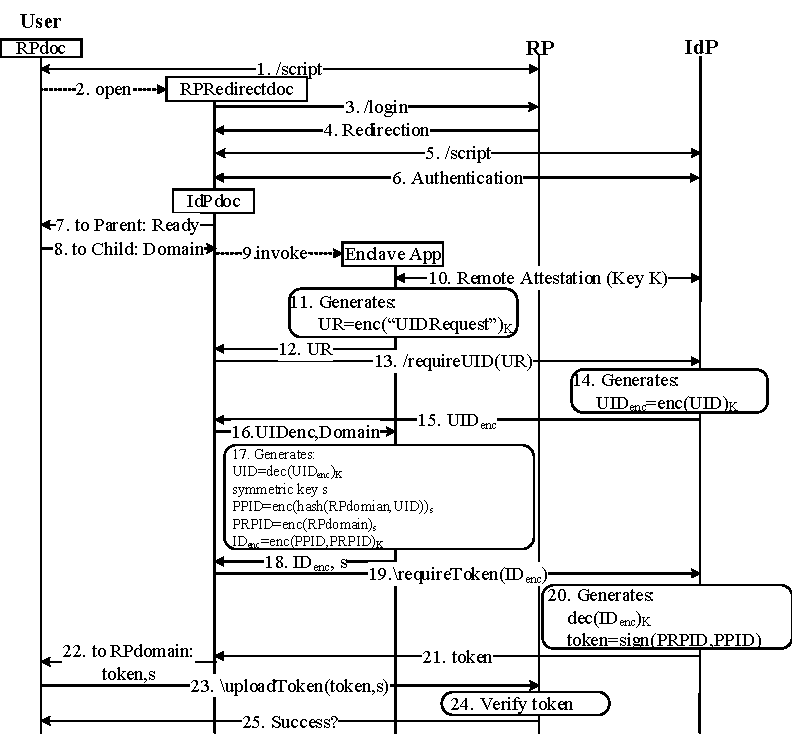
\includegraphics[width=0.95\linewidth]{fig/sgx-sso.pdf}
  \caption{The protocol flow of XXX.}
  \label{fig:XXX}
\end{figure}
The XXX is compatible with OIDC, besides that the IdP service is separated into user agent part and server part. 
The server part IdP service takes the responsibility of authenticating the user, retrieves the UID for each user, and issues the signed identity proof consisted the privacy-preserving RP and user identifier generated at user agent part IdP service.
The user agent part IdP service would obtain the UID from server part service, transform UID into the PPID, and encrypt the RPID and PPID with an one-time symmetric key to avoid IdP server digging out the RP's identity. As the enclave application is protected by SGX, it must not conduct any malicious behaviour. 

\subsection{XXX process}
In this section, we provide the detail protocol of XXX.

The process of XXX is depicted in detail in Figure~\ref{fig:XXX}.
The SSO process is started with the user's visit to an RP at her browser, and the browser downloads the RP script (step 1), which is used to conduct the behaviour defined by RP at user side. Then the RP script opens the new window with the RP login endpoint (step 2, 3). Then the user is redirected to the IdP server (step 4). It must be noticed that, the user cannot visit IdP at step 2,3 directly because of the $Referer$ attribute in HTTP header. While the script in origin A opens a new window with origin B, the HTTP request to B will carry the key value $Referer: A$. Therefore, the RP's domain is exposed to IdP. With HTML5, a special attribute for links in HTML was introduced, that the $ref="noreferrer"$ can be used to make $Referer$ header be suppressed. However, when such a link is used to open a new window, the new window does not have a handle on the opening window (opener) anymore. The handle is necessary for XXX to transmit messages between RP and IdP.



While the user is redirected to the IdP server, the IdP will retrieve the IdP script (step 5), witch is used to deal with the interaction with IdP server, RP script and enclave application.
And the IdP authenticates the user (step 6). After the IdP script is downloaded, it sends the ready signal to its opener (i.e., the RP window) (step 7). Then it will receive the $RPdomain$ from RP script for further process (step 8). There are some types of parameters required in OIDC protocol to be carried in the SSO request, such as $response\_type$ and $scope$. In this paper, we would not focus on these attributes, and only describe the necessary parameters. 

Then the user starts the SSO request to IdP (step 9). As the result, the user receives a $UID token$ from IdP (step 10), with which an enclave application can retrieve the user's real identifier UID from IdP server.

Then the IdP script invokes the enclave application with RP's domain and the $UID token$ (step 11). The enclave application requires the UID from IdP server with the UID token (step 12, 13). After receiving the UID, enclave application generates the symmetric key s, encrypts the RP's domain with key s as the transformed RP ID, and encrypts the hash of RP's domain and UID as the PPID (step 14). 

After the ID transformation, enclave application requires the IdP server to generate identity proof with $PRPID$ and $PPID$ (step 15). The IdP server signs the $token$ consisted of $PRPID$ and $PPID$ as the identity proof (step 16), and return it to enclave application (step 17). Then enclave application set the $token$ and key $s$ as the result of step 11 (step 18). The IdP script then sends the $token$ and $s$ to the origin $RPdomain$ through $postMessage$ (step 19). It guarantees that only the script running in the RP window can receive the $token$, which avoids the man-in-the-middle attack.

Finally, the RP script uploads the $token$ and key $s$ to RP server (step 20). The RP server firstly verifies the signature with IdP's public key, then generates the $PRPID$ with its domain and key $s$, and compared it with the one carried by $token$. If the two $PRPID$s are equal, RP decrypts the user's ID from $PPID$, and find out the related user information in its database (step 21). Then it returns the login result to user (step 22). 